\newpage
\subsection{Estrategia de seguridad y control de acceso}
\label{sec:seguridad-nube}

Para proteger la integridad de los datos y restringir el acceso a los recursos de la nube, se implementará una estrategia de seguridad perimetral y una gestión de identidad híbrida. 

La protección de los datos en tránsito se garantizará mediante AWS Certificate Manager (ACM), el cual aprovisionará y gestionará certificados SSL/TLS. Estos certificados se adjuntarán a los puntos de entrada públicos (Amazon API Gateway y Amazon CloudFront) para forzar que toda comunicación desde los clientes se realice exclusivamente bajo el protocolo HTTPS.

En cuanto al control de acceso, el sistema adoptará un enfoque híbrido para la autenticación:
\begin{itemize}
    \item \textbf{Plataforma Web:} Se utilizará Amazon Cognito para gestionar el grupo de usuarios administradores. Cognito proporcionará flujos seguros de inicio de sesión y emitirá tokens que la aplicación web enviará en cada petición.
    \item \textbf{Aplicación Móvil:} Dado el enfoque \textit{offline} del cliente móvil, el \textit{backend} (desarrollado en Micronaut) será el encargado de generar y validar firmas de JSON Web Tokens (JWT) propios. Esto aligerará la carga en el dispositivo móvil y permitirá una validación rápida y sin dependencias externas durante los procesos de sincronización.
\end{itemize}
Ambos tipos de tokens serán interceptados y validados por Amazon API Gateway antes de invocar cualquier función Lambda, protegiendo así la lógica de negocio subyacente.

\subsubsection{Almacenamiento y persistencia políglota}

El sistema requerirá manejar tanto información relacional estructurada como archivos binarios pesados. Para optimizar el rendimiento y los costos, se adoptará una arquitectura de persistencia políglota dividida en dos servicios:

\begin{enumerate}
    \item \textbf{Amazon RDS (PostgreSQL):} Actuará como la fuente de la verdad para los datos transaccionales. Almacenará los registros de usuarios, el inventario de árboles evaluados, la metadata de los reportes de detección y las configuraciones del sistema. Se eligió PostgreSQL por su robustez, cumplimiento ACID y capacidad para manejar consultas geoespaciales si el proyecto lo requiere en el futuro.
    \item \textbf{Amazon S3:} Proporcionará almacenamiento de objetos altamente escalable para datos no estructurados. Se configurarán \textit{buckets} con políticas de acceso estricto para almacenar tres tipos de artefactos: las imágenes fotográficas capturadas por el dispositivo móvil, las versiones compiladas de la aplicación web Angular y las versiones del modelo \texttt{.tflite} listas para su descarga.
\end{enumerate}

\subsubsection{Integración con Amazon SageMaker}

A diferencia de las arquitecturas clásicas de \textit{Machine Learning} en la nube, Amazon SageMaker no se utilizará para realizar inferencias en tiempo real, ya que esta tarea recaerá en el dispositivo móvil. En su lugar, SageMaker fungirá exclusivamente como un \textit{Model Registry} (Registro de Modelos).

El entrenamiento intensivo del modelo (basado en EfficientNet-B3 o YOLO) se ejecutará en equipos de cómputo locales. Una vez que el modelo alcance las métricas de precisión deseadas mediante evaluación con \textit{Scikit-learn}, sus pesos y arquitectura se subirán a Amazon SageMaker para versionarlo de manera formal. Finalmente, SageMaker orquestará la exportación del modelo al formato optimizado TensorFlow Lite (\texttt{.tflite}) y lo depositará en Amazon S3, quedando disponible para que los dispositivos móviles descarguen la actualización cuando dispongan de conexión a internet.

\subsubsection{Observabilidad y monitoreo centralizado}

Para garantizar la fiabilidad del entorno \textit{serverless}, se implementará una capa transversal de observabilidad utilizando Amazon CloudWatch. Este servicio centralizará la telemetría del sistema sin requerir la instalación de agentes adicionales.

CloudWatch recolectará de manera automática los registros de ejecución (\textit{logs}) emitidos por las funciones AWS Lambda en Java/Micronaut, facilitando la depuración de errores. Asimismo, monitoreará las métricas críticas de Amazon API Gateway, tales como la latencia de las peticiones, la tasa de errores HTTP 4xx/5xx y el volumen de tráfico. Se configurarán alarmas automatizadas para notificar a los administradores ante cualquier anomalía operativa, como un pico inusual en los tiempos de arranque (\textit{cold starts}) o intentos masivos de acceso denegado.

\subsubsection{Entorno de desarrollo y automatización (CI/CD)}

El ciclo de vida del desarrollo de \textit{software} integrará prácticas de DevOps para asegurar transiciones seguras entre el código local y la nube. 

A nivel local, los desarrolladores utilizarán contenedores \textbf{Docker} para levantar instancias aisladas de PostgreSQL, asegurando la paridad entre el entorno de desarrollo y producción. Como paso intermedio, se configurará una \textbf{Raspberry Pi} que actuará como un servidor \textit{on-premise} de pruebas e integración, permitiendo validar el comportamiento de la aplicación Micronaut en un entorno Linux real antes de impactar los servicios de AWS.

El despliegue hacia la nube estará completamente automatizado mediante \textbf{GitHub Actions}. Se construirá un \textit{pipeline} de Integración y Despliegue Continuo (CI/CD) que reaccionará a los cambios en la rama principal del repositorio. Las etapas automatizadas incluirán: la compilación del código fuente, la ejecución de pruebas unitarias, el empaquetado del artefacto Java 21 y, finalmente, la actualización automática del código en AWS Lambda mediante la interfaz de línea de comandos (AWS CLI).

\begin{figure}[H]
    \centering
       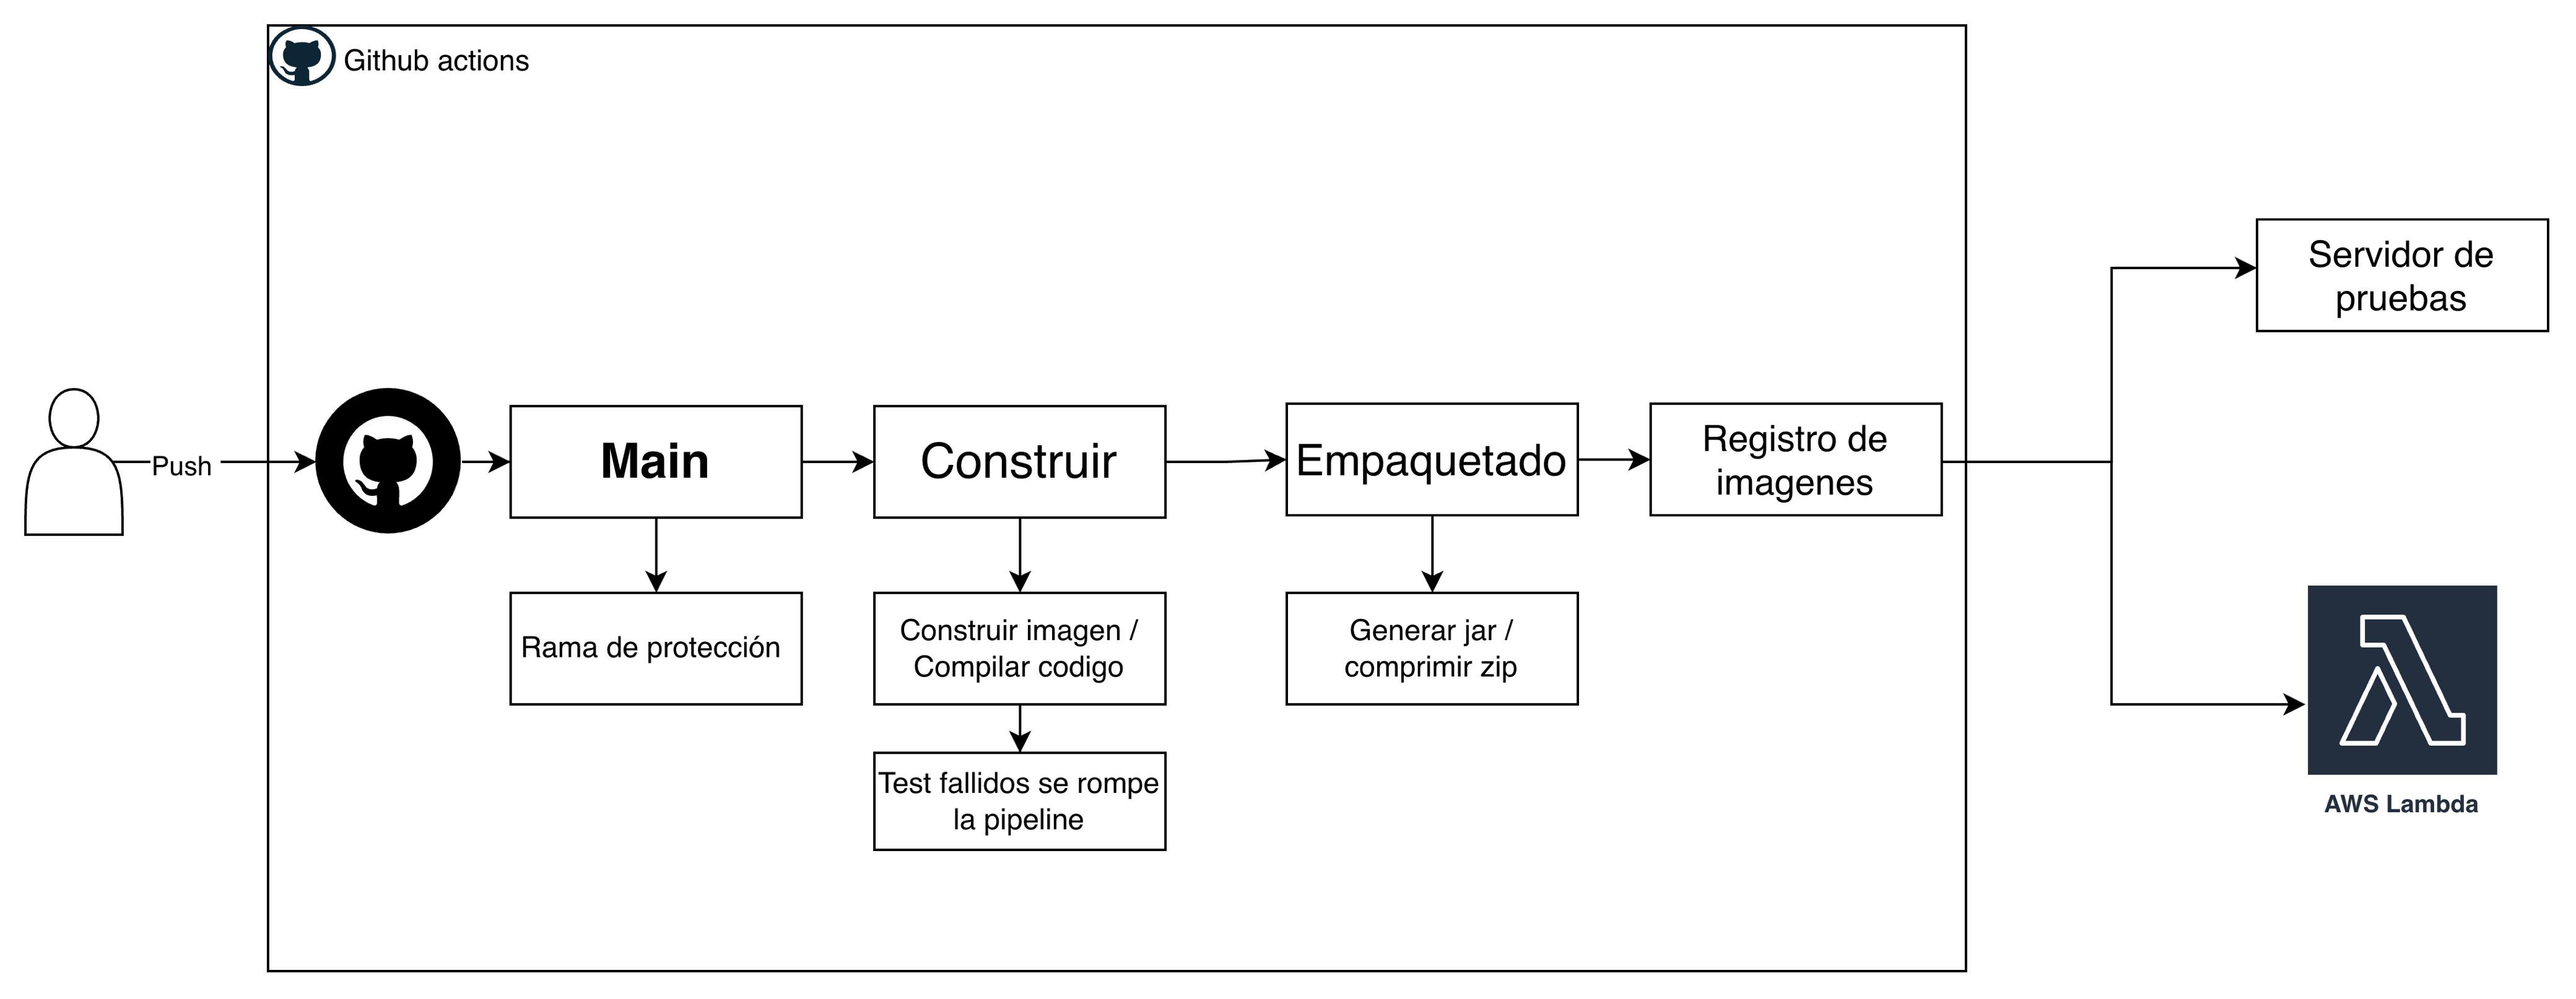
\includegraphics[width=0.95\textwidth]{images/C8/ci_cd.jpeg}
    \caption{Flujo de Integración y Despliegue Continuo (CI/CD).}
    \label{fig:pipeline-cicd}
\end{figure}


\subsubsection{Flujos principales de comunicación}

El flujo de información más crítico de la arquitectura es el proceso asíncrono de sincronización entre el cliente móvil \textit{offline} y la nube. Este proceso se ejecutará de manera secuencial siguiendo los principios de las arquitecturas basadas en eventos:

\begin{enumerate}
    \item El dispositivo móvil, tras operar en campo sin red, detecta conexión a internet e inicia el proceso de sincronización leyendo los registros locales almacenados en SQLite.
    \item El cliente (mediante Retrofit) realiza una petición REST segura al \textit{endpoint} correspondiente en Amazon API Gateway, adjuntando el JWT propio en las cabeceras de autorización.
    \item API Gateway intercepta la petición y verifica la firma del token. Si es válido, canaliza el cuerpo de la petición (texto e imágenes codificadas) hacia AWS Lambda.
    \item La función Lambda inicializa el contexto de Micronaut. Extrae las imágenes, las decodifica y las transmite hacia Amazon S3, obteniendo como respuesta una URL (URI) permanente.
    \item Posteriormente, Lambda construye el objeto de dominio del reporte, asocia la URL de S3 al registro y lo persiste de manera transaccional en Amazon RDS (PostgreSQL).
    \item Finalmente, Lambda retorna un código HTTP 200 OK hacia la aplicación móvil, la cual procede a marcar los registros locales como "sincronizados" para evitar duplicidades futuras.
\end{enumerate}

\begin{figure}[H]
    \centering
      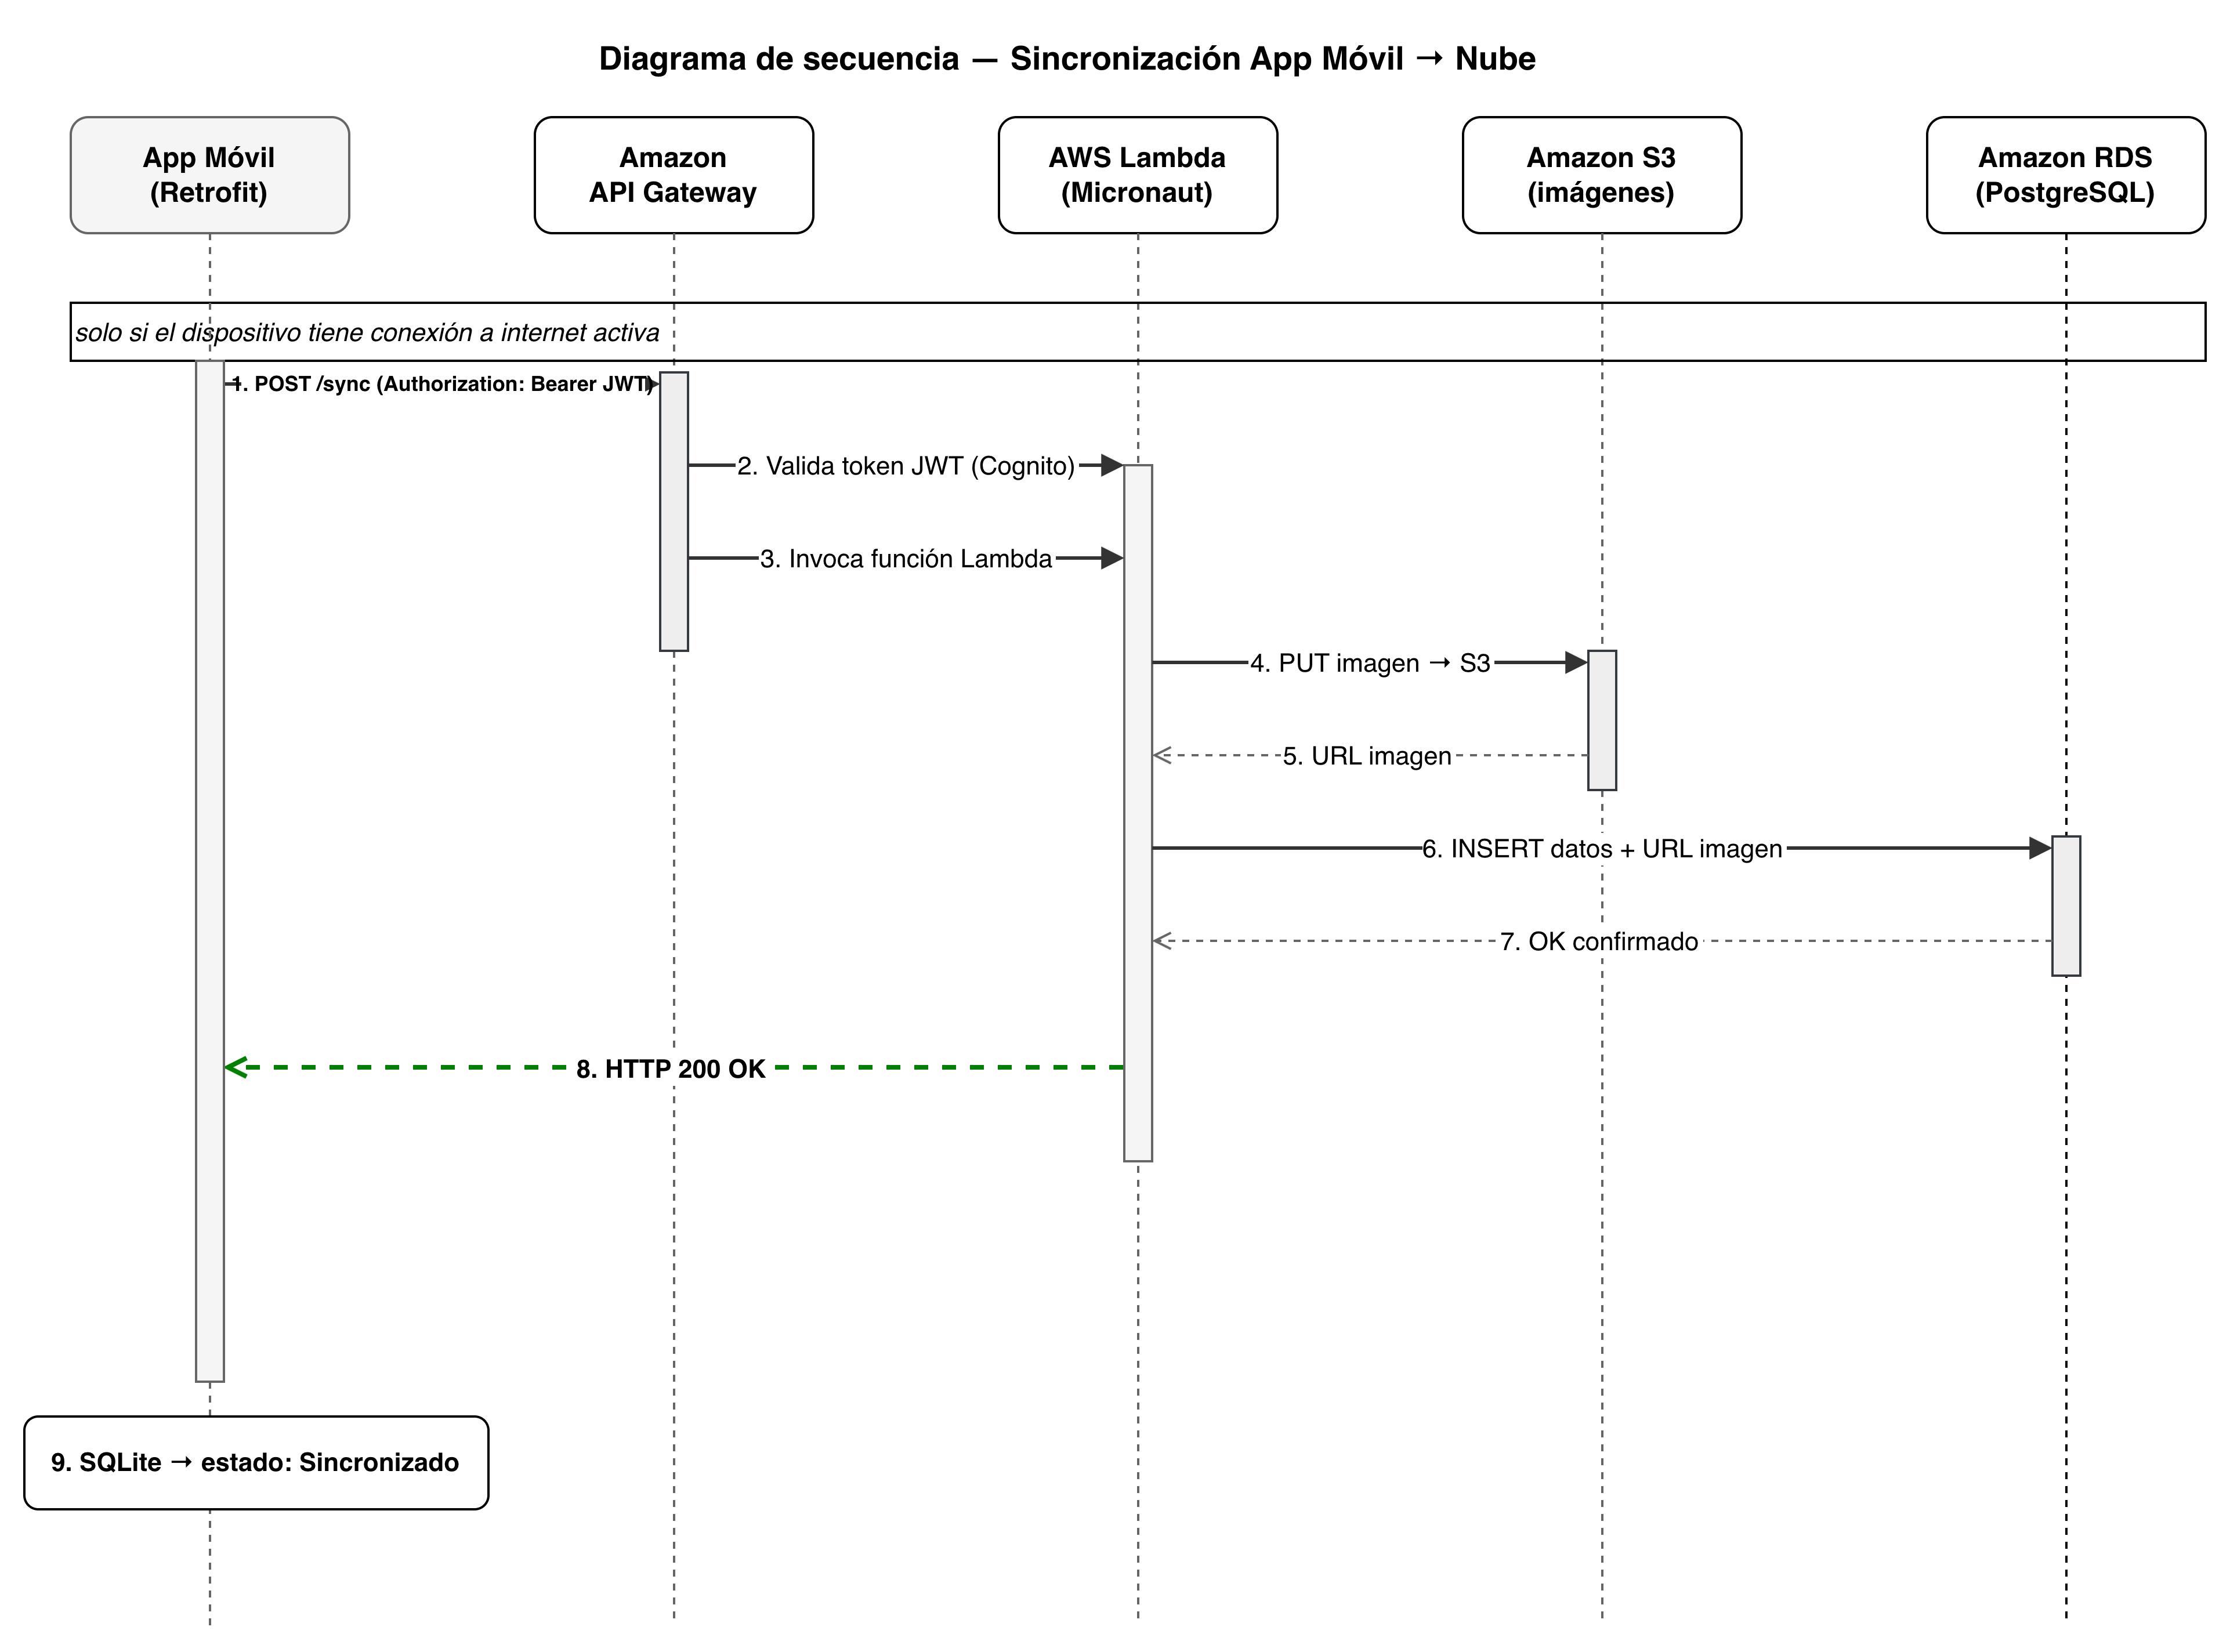
\includegraphics[width=0.95\textwidth]{images/C8/secuencia_movil.jpeg}
    \caption{Diagrama de secuencia del proceso de sincronización de datos.}
    \label{fig:secuencia-sincronizacion}
\end{figure}

\subsubsection{Estructura interna del backend (Clean Architecture)}

El \textit{backend} alojado en AWS Lambda se implementará utilizando el
lenguaje Java 21 acompañado del \textit{framework} Micronaut. La decisión
de usar Micronaut responde a su capacidad para resolver la inyección de
dependencias en tiempo de compilación (\textit{Ahead of Time - AoT}),
eliminando la sobrecarga en tiempo de ejecución característica de
\textit{frameworks} tradicionales como Spring, lo cual es vital para
mantener la latencia baja en un modelo \textit{serverless}.

Para asegurar la alta cohesión, el bajo acoplamiento y la facilidad de
mantenimiento, la base de código se estructurará siguiendo los principios
de \textit{Clean Architecture} (Arquitectura Limpia). Las dependencias del
código apuntarán exclusivamente hacia adentro, organizándose en las
siguientes capas concéntricas:

\begin{itemize}
    \item \textbf{Capa de Dominio (\textit{Domain}):} Constituirá el núcleo
    del sistema. Contendrá las entidades de negocio puras (\texttt{Deteccion},
    \texttt{Arbol}, \texttt{Usuario}, \texttt{Captura}) y sus invariantes,
    sin dependencias hacia ninguna tecnología o librería externa. También
    define las interfaces abstractas de repositorio (\texttt{DeteccionRepository},
    \texttt{ArbolRepository}) que las capas externas deberán implementar,
    aplicando el principio de inversión de dependencias.

    \item \textbf{Capa de Casos de Uso (\textit{Use Cases}):} Orquestará
    el flujo de datos desde y hacia las entidades. Implementará la lógica
    de la aplicación, como registrar un nuevo hallazgo geolocalizado,
    procesar la sincronización masiva proveniente del dispositivo móvil o
    consultar el historial de detecciones de un árbol específico. Cada caso
    de uso es una clase independiente con una única responsabilidad, lo que
    facilita las pruebas unitarias aisladas.

    \item \textbf{Capa de Adaptadores (\textit{Interface Adapters}):} Actuará
    como traductora entre el mundo exterior y los casos de uso. Aquí residirán
    los controladores REST (\texttt{SyncController}, \texttt{DetectionController},
    \texttt{TreeController}, \texttt{UserController}) que transforman las
    peticiones HTTP de Amazon API Gateway en objetos de dominio, así como
    los \textit{mappers} que convierten entre entidades y DTOs de transferencia.

    \item \textbf{Capa de Infraestructura (\textit{Infrastructure}):} Será
    la capa más externa, encargada de proveer las implementaciones concretas.
    Contendrá los módulos de Micronaut Data JPA e Hibernate para la persistencia
    en PostgreSQL sobre Amazon RDS, la integración del SDK de AWS para la
    carga de imágenes en Amazon S3, y los componentes de seguridad encargados
    de la validación de tokens JWT. También incluirá la configuración de
    Amazon CloudWatch para el monitoreo de logs y métricas en tiempo de
    ejecución.
\end{itemize}

La estructura de paquetes del proyecto refleja directamente esta separación
de capas:

\begin{verbatim}
com.descortezadores.backend/
  domain/
    entities/          (Deteccion, Arbol, Usuario, Captura)
    repositories/      (interfaces abstractas)
    rules/             (invariantes y reglas de negocio)
  usecases/
    sync/              (SyncDeteccionUseCase)
    detection/         (RegistrarDeteccionUseCase)
    history/           (ConsultarHistorialUseCase)
  adapters/
    controllers/       (SyncController, DetectionController)
    mappers/           (DeteccionMapper, ArbolMapper)
    repositories/      (DeteccionRepositoryImpl, S3ImageRepository)
  infrastructure/
    persistence/       (Micronaut Data JPA, Hibernate)
    aws/               (S3Client, CognitoValidator)
    security/          (JwtValidator)
    config/            (MicronautConfig, DataSourceConfig)
\end{verbatim}

Esta organización garantiza que cualquier cambio en la infraestructura,
como migrar de PostgreSQL a Aurora o cambiar el proveedor de almacenamiento,
no afecte la lógica de negocio ni los casos de uso del sistema.

\begin{figure}[H]
    \centering
      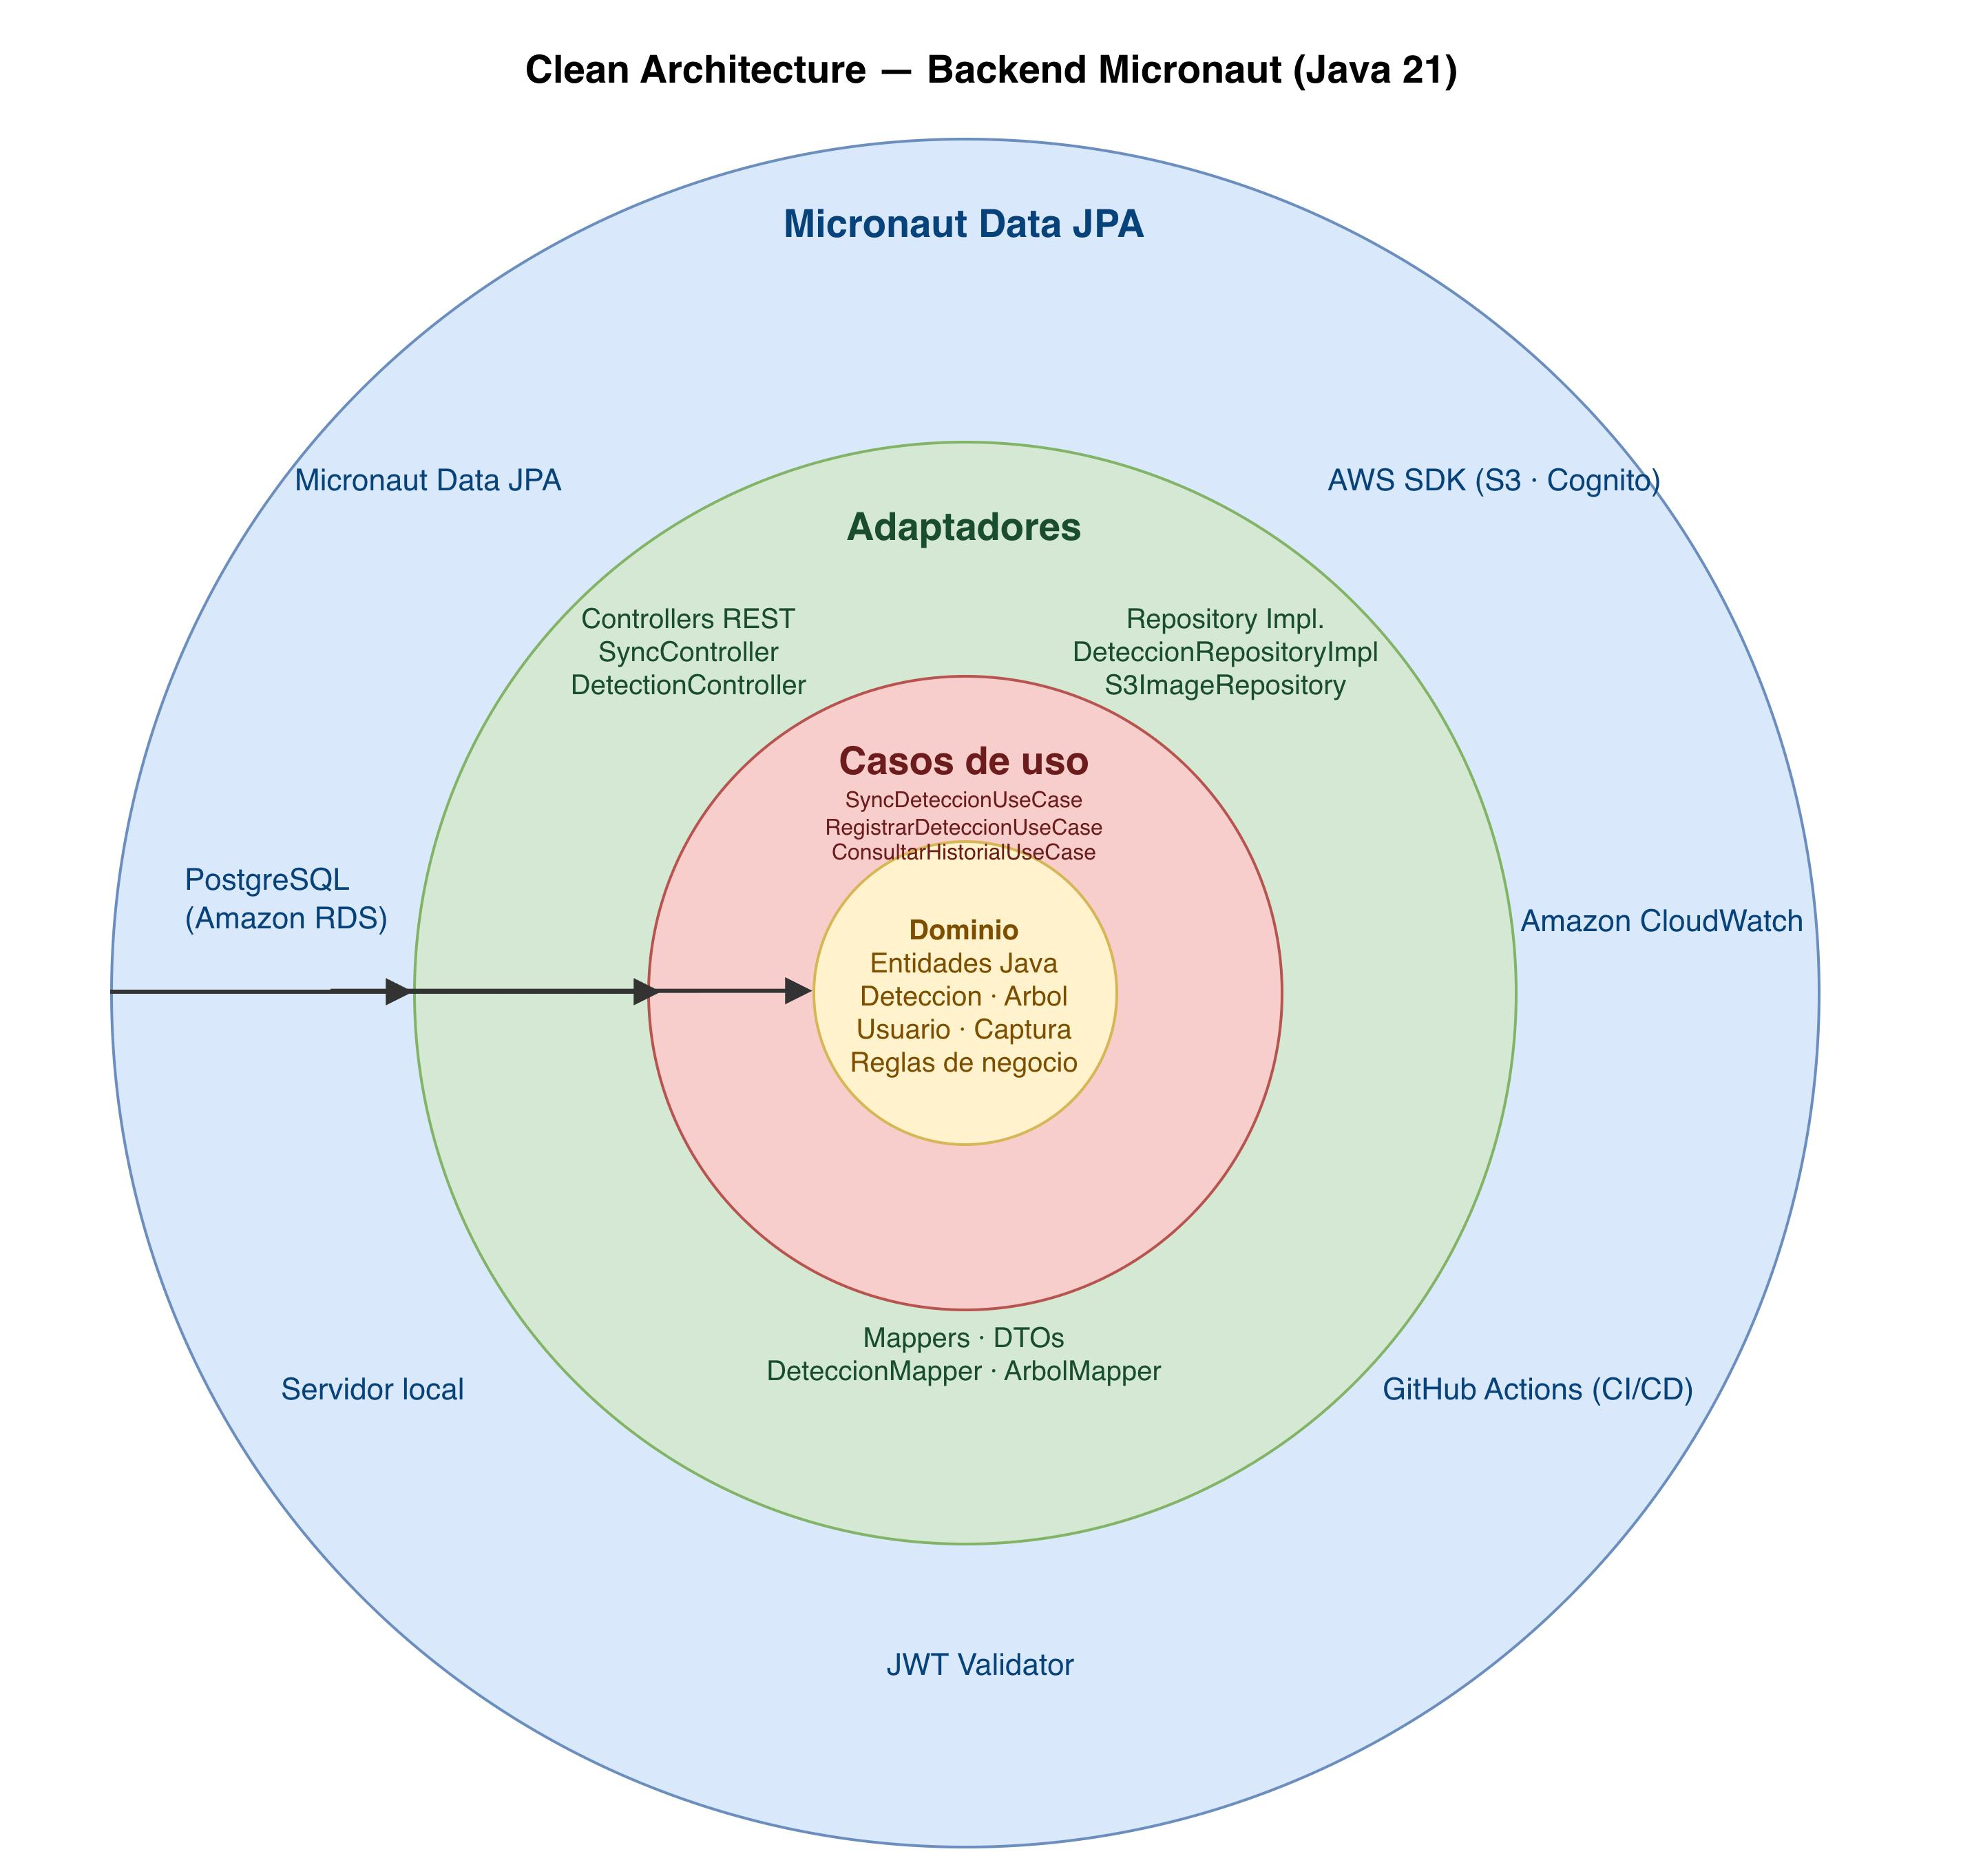
\includegraphics[width=0.95\textwidth]{images/C8/clean_architecture.jpeg}
    \caption{Estructura en capas del \textit{backend} basada en
    \textit{Clean Architecture}.}
    \label{fig:clean-architecture}
\end{figure}